\section[Visualization I: Orthogonal coordinate systems]{Visualization I\\Orthogonal coordinate systems}
To help orient our eyes to the different operations, we created the letter F by simply identifying the vertices and tracking the movement of these points. (See figure \eqref{fig:8:fdots}.) Each point represents a vector and we act on these vectors with the orthogonal matrix of interest to catalog the effects of different basis matrices in $\real{2}$.
\begin{SCfigure}
  \centering
  \includegraphics[ width = 1.5in ]{pdf/"ch 08"/"for real"/"f with dots"}
  \caption[A collection of points used to study matrix actions]{A collection of points used to study matrix actions. The shading helps to unify the points and to enunciate the chirality of the system.}
\label{fig:8:fdots}
\end{SCfigure}


Start with the rotations by $\pihalf$. Notice that the exponential operator maps multiplication into addition:
\begin{equation}
  e^{i \theta_{1}} e^{i \theta_{2}} = e^{i \paren{\theta_{1} + \theta_{1}}}.
\end{equation}
As we saw in the homework problem in chapter 0?, the rotation operator is the exponential operator in disguise. We see that this matrix also maps multiplication into addition:
\begin{equation}
  \RR{\theta_{1}}\RR{\theta_{2}} = \RR{\theta_{1} + \theta_{2}}
\end{equation}
In the following figure we will look at a sequence of successive rotations by $\pihalf$. We can compute any rotation directly using the rotation matrix and the proper value for the angle $\theta$, or we could compound the result:
\begin{equation}
  \begin{array}{llcl}
     \RR{\pihalf} & \itwo &=& \RR{\pihalf} \\
     \RR{\pihalf} & \RR{\pihalf} &=& \RR{\pi} \\
     \RR{\pihalf} & \RR{\pi} &=& \RR{\frac{3}{2}\pi} \\
     \RR{\frac{3}{2}\pi} & \RR{\pihalf} &=& \RR{2\pi}.
  \end{array}
\end{equation}
This rotation sequence is shown in figure \eqref{tab:8:catalog}. The way to read these figures is shown in table \eqref{tab:8:seq}.
\begin{table}[htdp]
\begin{center}
\begin{tabular}{m{0.25in}m{0.45in}m{0.5in}m{0.65in}m{0.5in}}
%%%
$\RR{\pihalf}$  & acts on & 
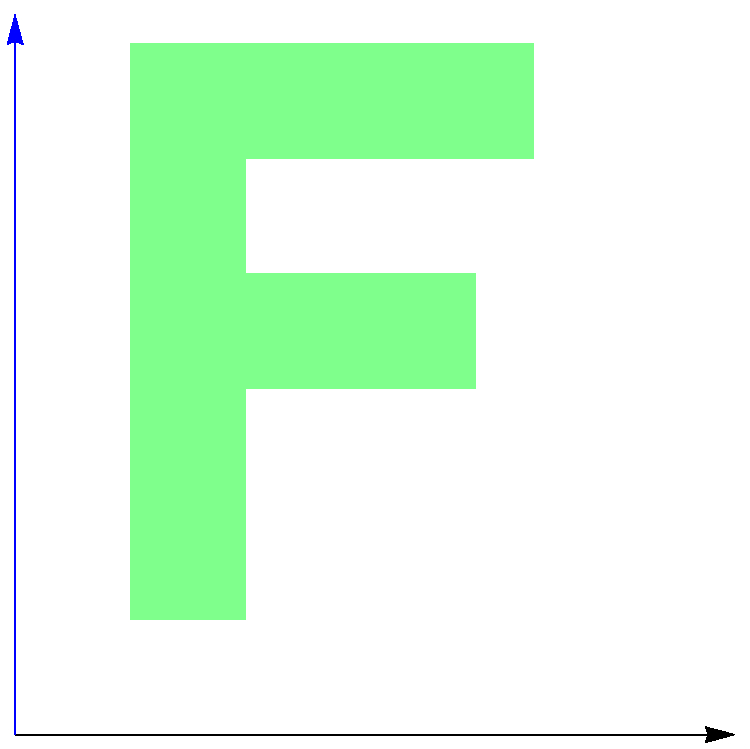
\includegraphics[ width = 0.5in ]{pdf/"ch 08"/"for real"/Ia} & to produce & 
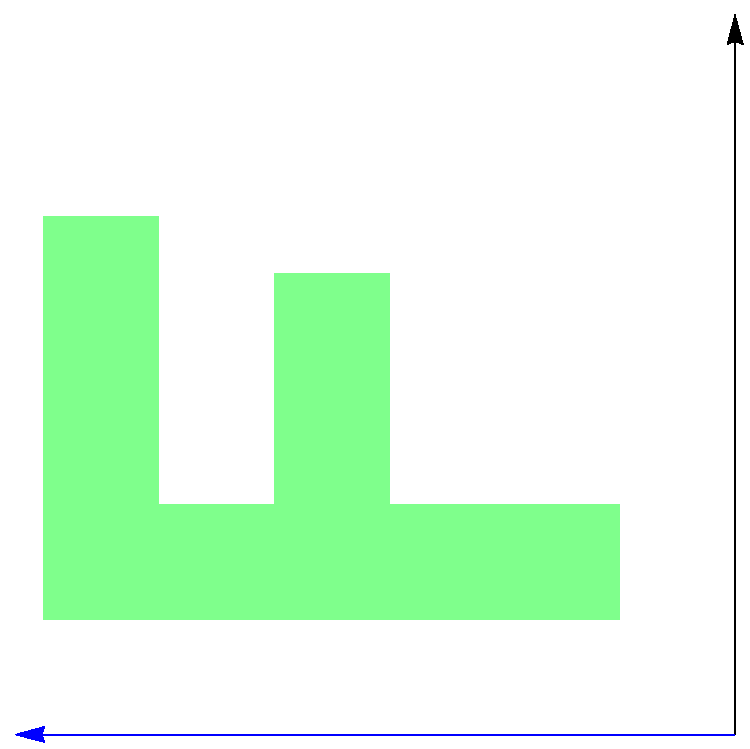
\includegraphics[ width = 0.5in ]{pdf/"ch 08"/"for real"/IIa} \\
%%%
$\RR{\pihalf}$  & acts on & 
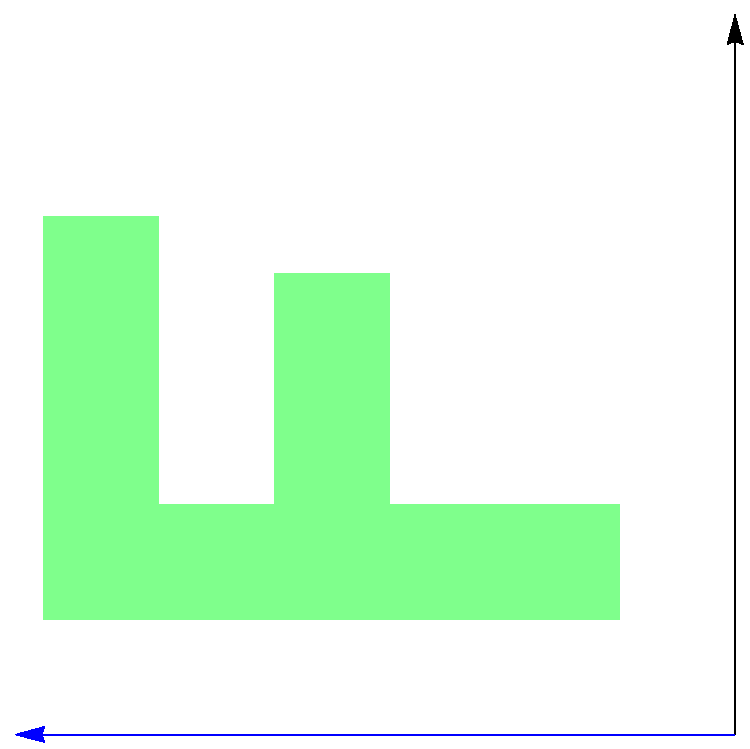
\includegraphics[ width = 0.5in ]{pdf/"ch 08"/"for real"/IIa} & to produce & 
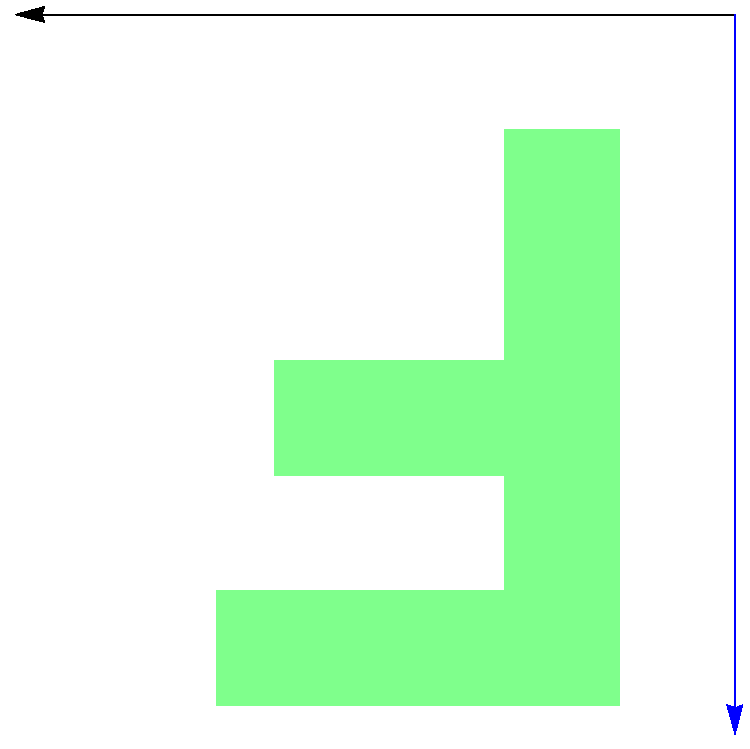
\includegraphics[ width = 0.5in ]{pdf/"ch 08"/"for real"/IIIa} \\
%%%
$\RR{\pihalf}$  & acts on & 
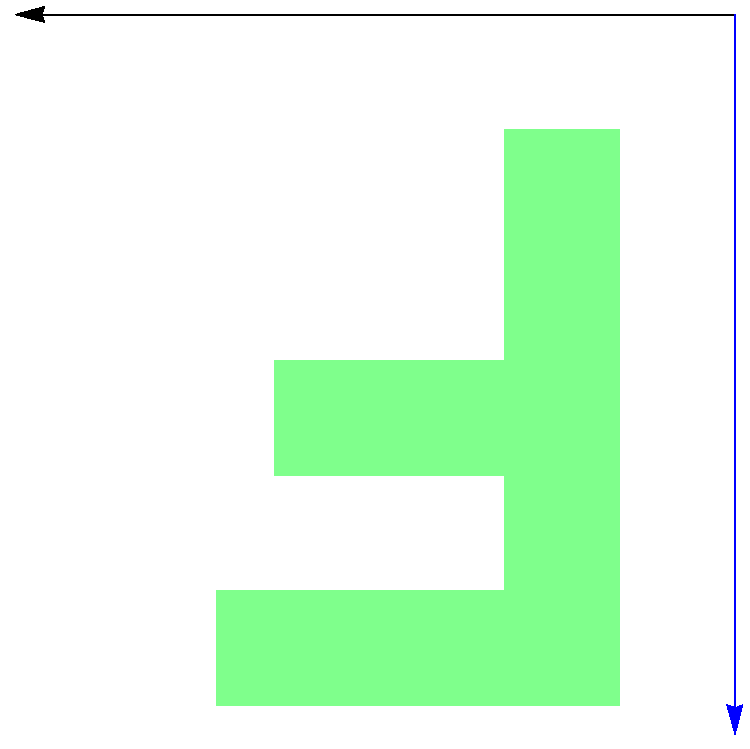
\includegraphics[ width = 0.5in ]{pdf/"ch 08"/"for real"/IIIa} & to produce & 
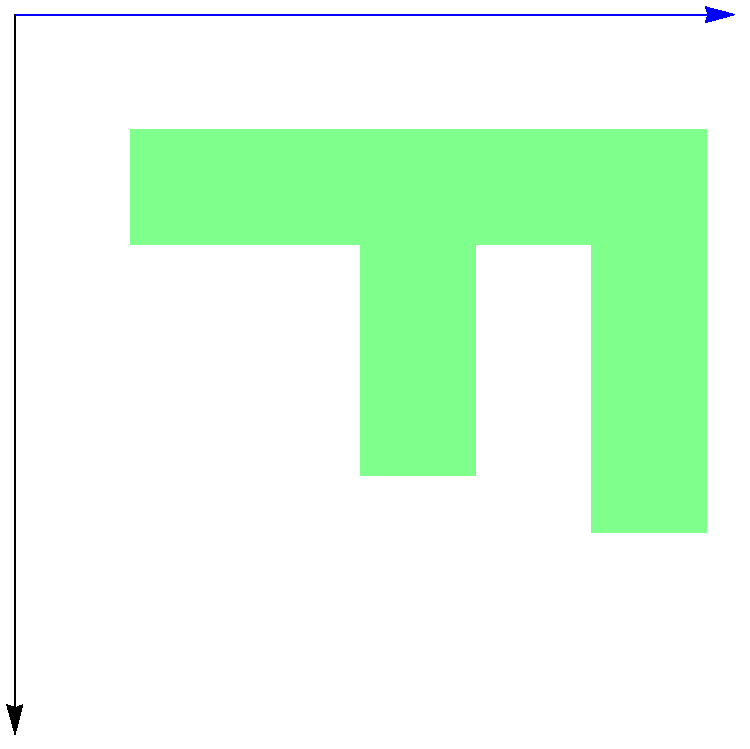
\includegraphics[ width = 0.5in ]{pdf/"ch 08"/"for real"/IVa} \\
%%%
$\RR{\pihalf}$  & acts on & 
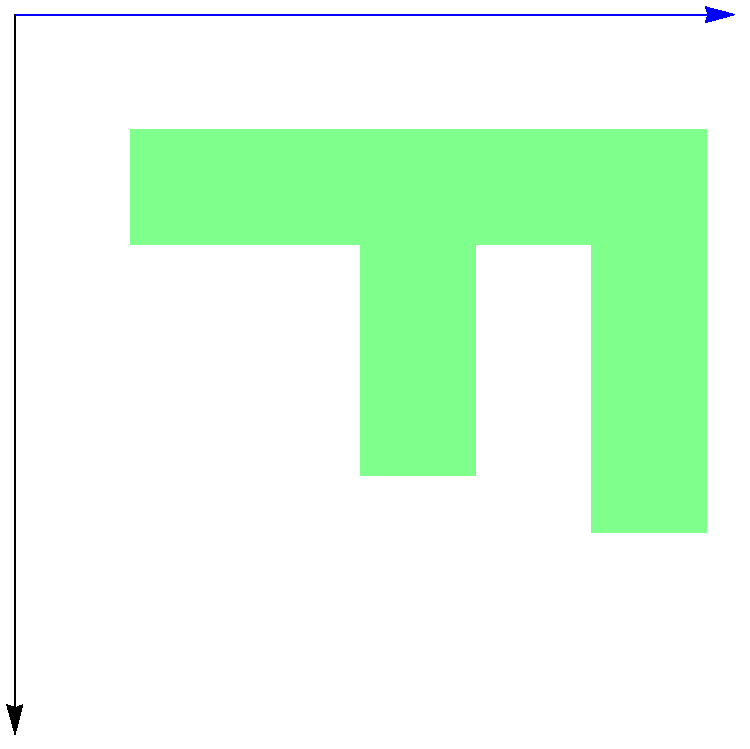
\includegraphics[ width = 0.5in ]{pdf/"ch 08"/"for real"/IVa} & to produce & 
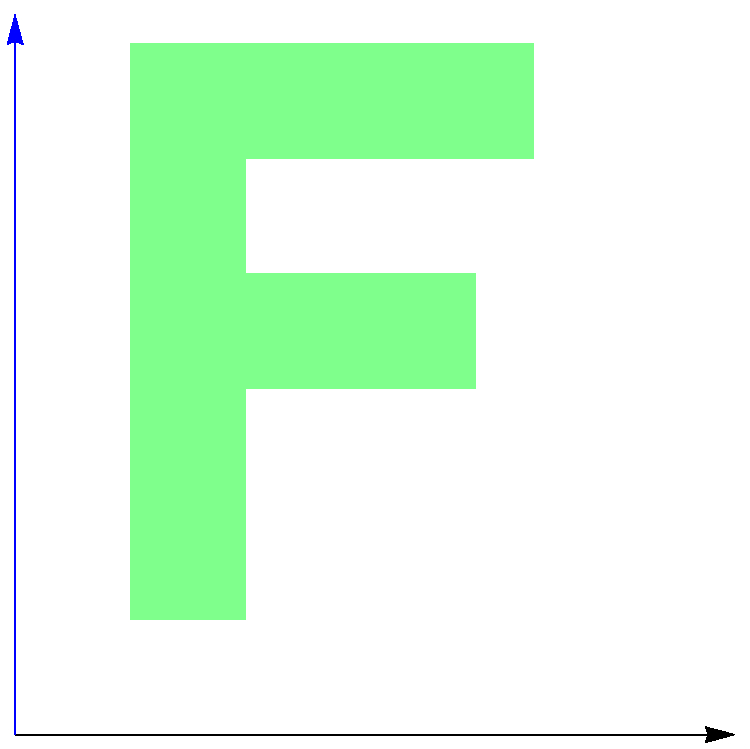
\includegraphics[ width = 0.5in ]{pdf/"ch 08"/"for real"/Ia} \\
%%%
\end{tabular}
\end{center}
\caption[Successive rotations by $\pihalf$]{Successive rotations by $\pihalf$. The domain matrices in the \svdl \ are often examples of rotation matrices.}
\label{tab:8:seq}
\end{table}%

to say that
\begin{table}[htdp]
\begin{center}
\begin{tabular}{m{0.1in}m{0.75in}m{1.15in}c|m{0.1in}m{0.75in}m{1.15in}}
  & matrix & action & \qquad && matrix & action \\\hline
%%%
  (a) & $\itwo$ & 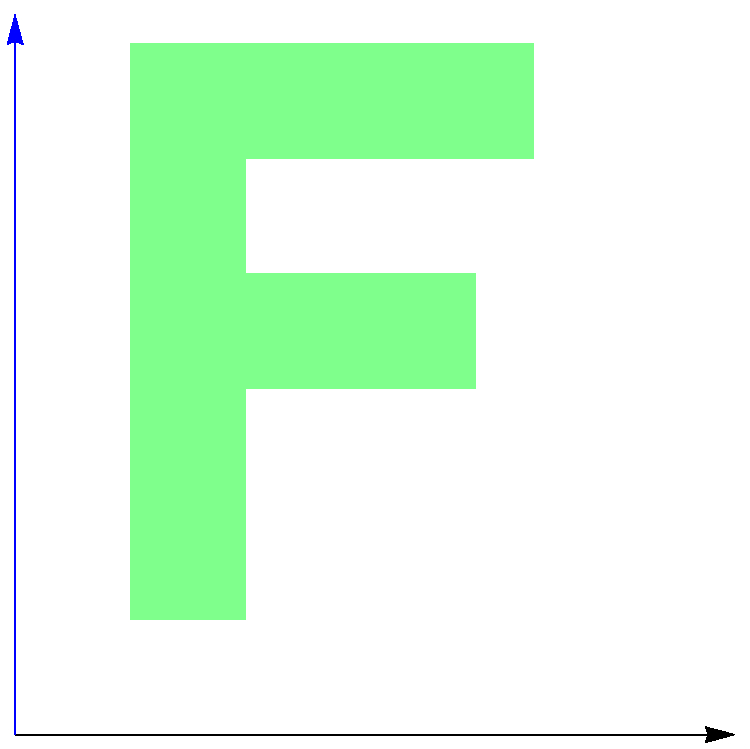
\includegraphics[ width = 1.25in ]{pdf/"ch 08"/"for real"/Ia} &&
  (b) & $\mat{cr}{0 & -1 \\ 1 & 0}$ & 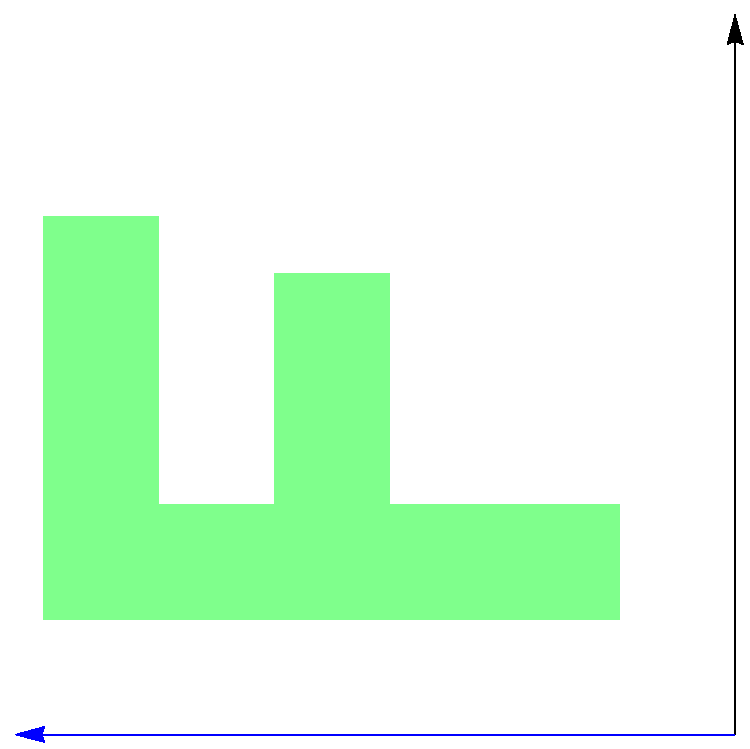
\includegraphics[ width = 1.25in ]{pdf/"ch 08"/"for real"/IIa} \\[25pt]
%%%
  (c) & $\mat{rr}{-1 & 0 \\ 0 & -1}$ & 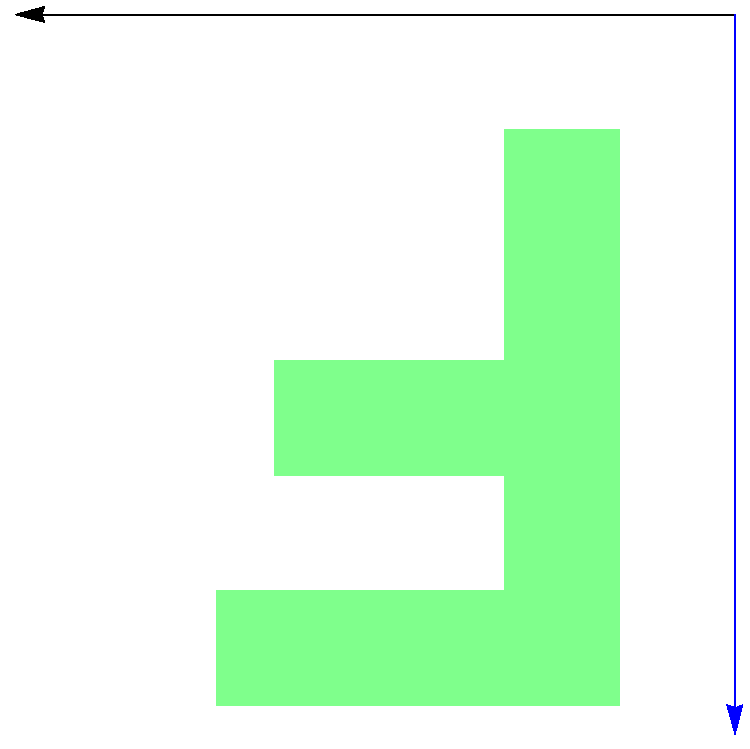
\includegraphics[ width = 1.25in ]{pdf/"ch 08"/"for real"/IIIa} &&
  (d) & $\mat{rc}{0 & 1 \\ -1 & 0}$ & 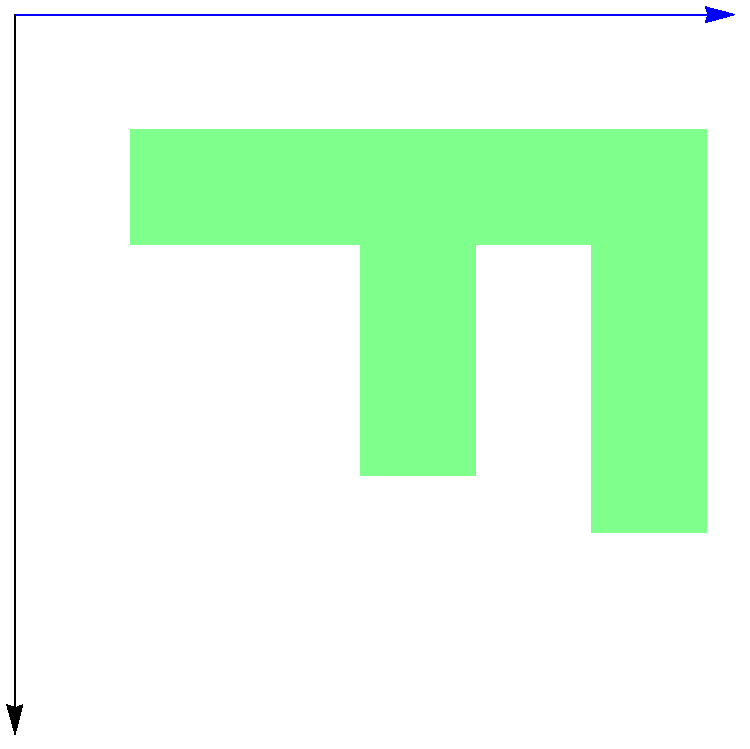
\includegraphics[ width = 1.25in ]{pdf/"ch 08"/"for real"/IVa} \\
%%%
\end{tabular}
\end{center}
\label{tab:8:catalog}
\caption[Successive rotations by $\pihalf$]{Successive rotations by $\pihalf$. None of these actions change the chirality of the image.}
\end{table}%
A fundamental truth emerges: rotations cannot change chirality. You are above the axis and the plane is spinning about the origin. You will always see the green color from the top.

Next, we consider reflections. We will reflect through the $x-$axis, the $y-$axis, the origin and an arbitrary line. Some of the reflections will change the chirality of the image.
\begin{table}[htdp]
\begin{center}
\begin{tabular}{m{0.1in}m{0.75in}m{1.15in}c|m{0.1in}m{0.75in}m{1.15in}}
  & matrix & action & \qquad && matrix & action \\\hline
%%%
  (a) & $\mat{cr}{1 & 0 \\ 0 & -1}$ & 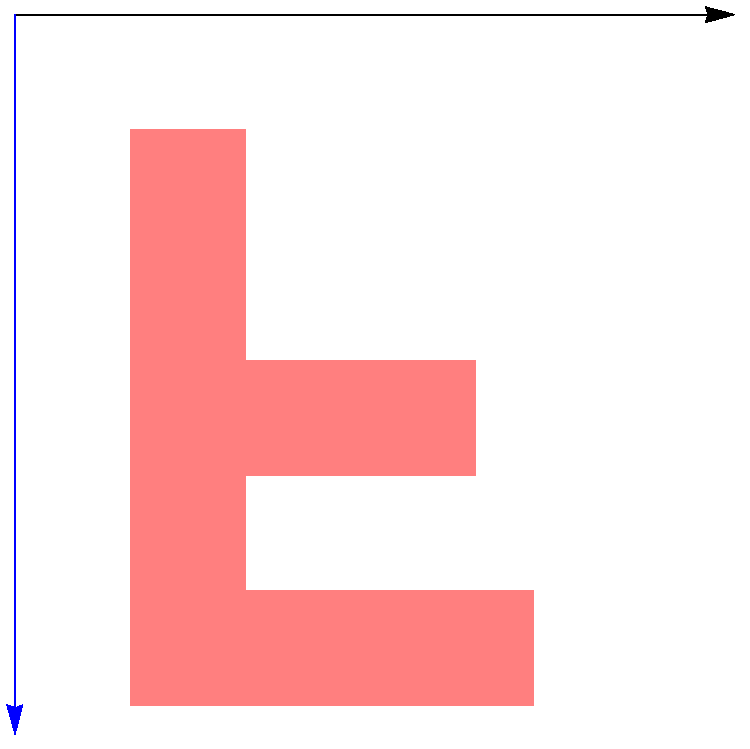
\includegraphics[ width = 1.25in ]{pdf/"ch 08"/"for real"/IVb} &&
  (b) & $\mat{rc}{-1 & 0 \\ 0 & 1}$ & 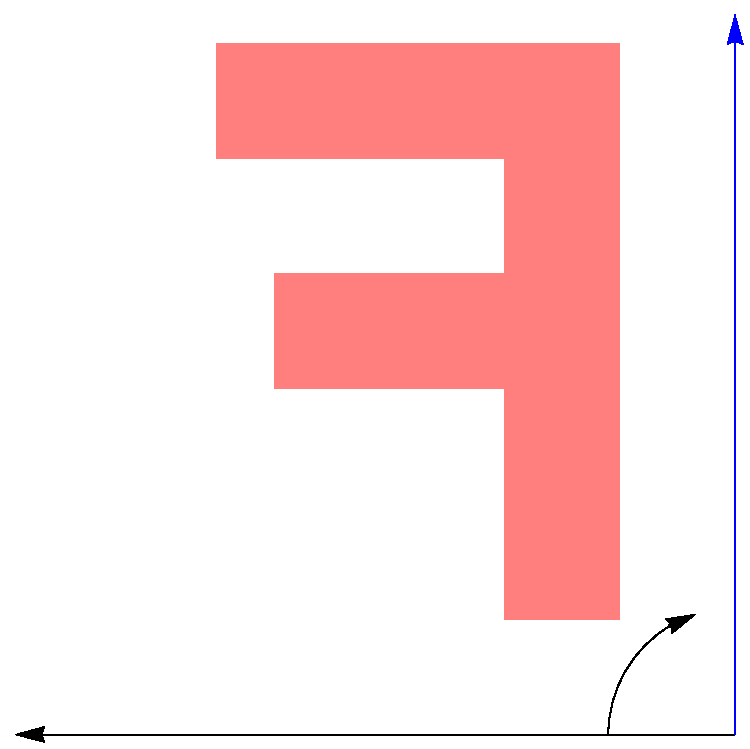
\includegraphics[ width = 1.25in ]{pdf/"ch 08"/"for real"/IIb} \\[25pt]
%%%
  (c) & $\mat{rr}{-1 & 0 \\ 0 & -1}$ & 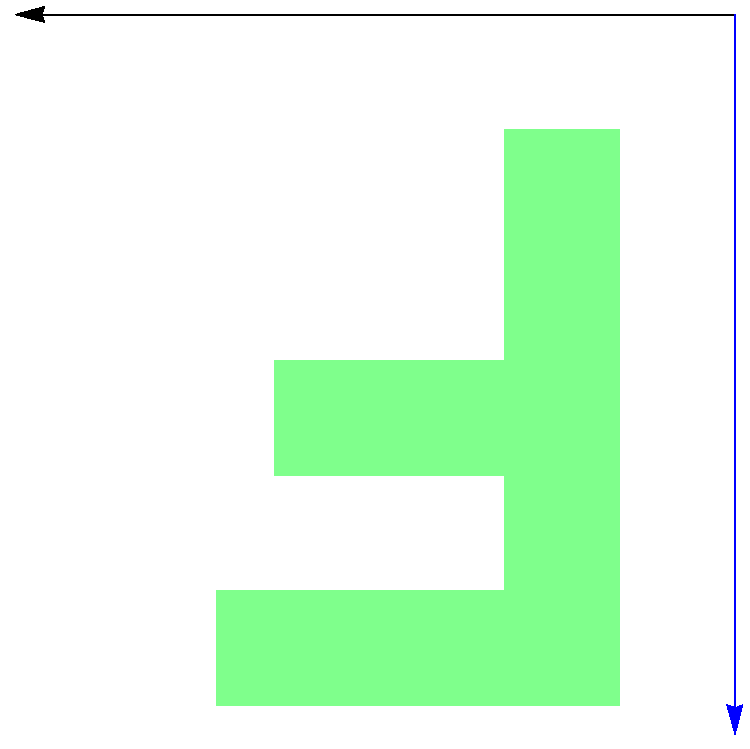
\includegraphics[ width = 1.25in ]{pdf/"ch 08"/"for real"/IIIa} &&
  (d) & $\mat{cc}{0 & 1 \\ 1 & 0}$   & 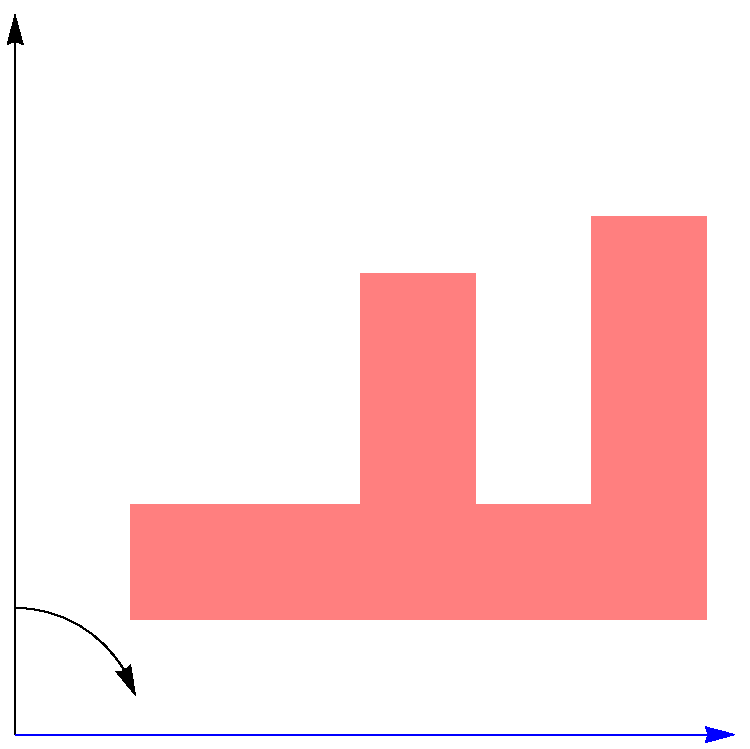
\includegraphics[ width = 1.25in ]{pdf/"ch 08"/"for real"/Ib} \\
%%%
\end{tabular}
\end{center}
\label{tab:8:reflections}
\caption[Primary reflections in the plane]{Primary reflections in the plane. Here we (a) reflect through the $x-$axis (complex conjugation), (b) the $y-$axis, (c) the origin, and finally (d), a reflection through the line $y=x$. Some reflections do change the chirality of the image.}
\end{table}%

Using the perspective of rotations and reflections we have covered all eight possible matrix combinations of the form
\begin{equation}
  \mat{rr}{\pm 1 & 0 \\ 0 & \pm}, \quad \mat{rr}{0 & \pm 1 \\ \pm 1 & 0}.
\end{equation}
Notice the dual nature of figures \eqref{tab:8:catalog} (c) and  \eqref{tab:8:reflections} (c). This tells us the the rotation by $\pi$ is equivalent to a reflection through the origin. The moral of the story is that there are more than one way to interpret these matrices, especially when it comes to compositions. This leaves us with rotations through arbitrary angles, reflections through arbitrary lines and their permutations. Two examples are shown below in figure \eqref{fig:8:rotref}.
\begin{figure}[htbp] %  figure placement: here, top, bottom, or page
   \centering
   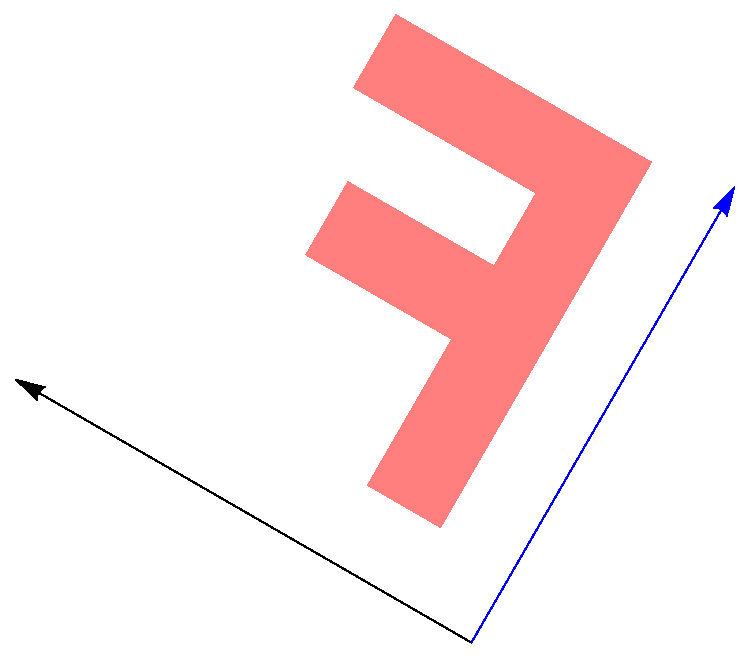
\includegraphics[ width = 2.25in ]{pdf/"ch 08"/"for real"/ref} \qquad
   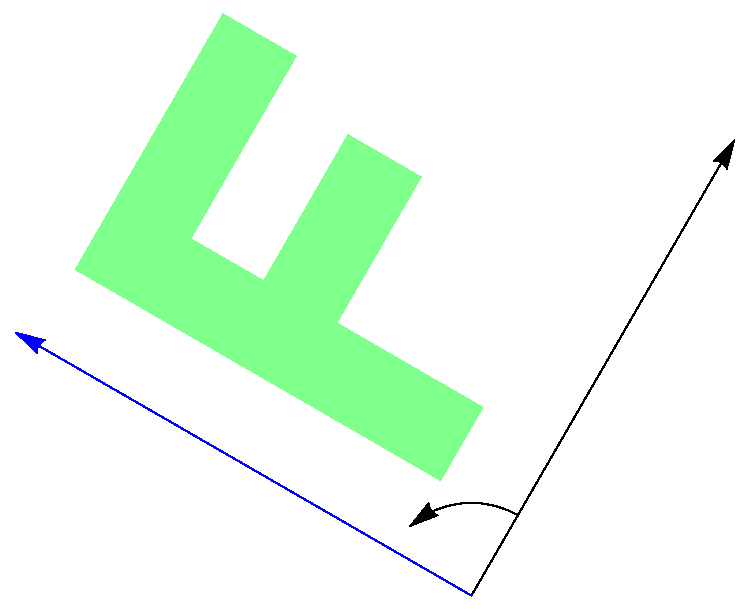
\includegraphics[ width = 2.25in ]{pdf/"ch 08"/"for real"/rot} 
   \caption[An arbitrary rotation and an arbitrary reflection.]{An arbitrary rotation (left) and an arbitrary reflection (right). Rotations never change the chirality of the image; single reflections always change the chirality of the image. Notice that both of the letters F share the same origin and axes. The green F is viewed from above the plane, the red F viewed from below.}
   \label{fig:8:rotref}
\end{figure}

But keep in mind the simple fact that the column vectors of an orthogonal matrix will always lie on the unit circle and they will always be orthogonal. For an orthogonal matrix
\begin{equation}
  \Q{} = \mat{cc}{ q_{1} & q_{2}} \in \real{2}
\end{equation}
this means that
\begin{enumerate}
\item $\normt{ q_{1} } = \normt{ q_{2} } = 1$,
\item $q_{1}q_{2}^{\TT}= 0.$
\end{enumerate}
Homework: change this for complex, show row vectors also satisfy this.

 
\endinput